\documentclass[11pt,a4paper]{report}

\usepackage[margin=2cm]{geometry}
\usepackage[matrix,frame,arrow]{xypic}
\usepackage{enumitem} %with options [nosep] or [noitemsep]  after \begin{enumerate} etc.
\usepackage[usenames, dvipsnames]{xcolor}
\usepackage{amsmath}
\usepackage{amssymb}
\usepackage{amsthm}
\usepackage{mathrsfs}
\usepackage[alphabetic]{amsrefs}
\usepackage[normalem]{ulem}  %does not alter \emph;   \sout{strike out}; \xout{cross out}
\usepackage[braket,qm]{qcircuit}
\usepackage{caption}  %use \captionsetup{justification=centering} within figure environment
\usepackage{appendix}
\usepackage{yfonts}  %use \textgoth
\def\initdefault{yinit}
\usepackage{tikz}
%\usetikzlibrary{quantikz}  %see http://mirror.aarnet.edu.au/pub/CTAN/graphics/pgf/contrib/quantikz/quantikz.pdf
\usetikzlibrary{matrix,arrows.meta}
%\usepackage{relsize}
%\renewcommand\RSlargest{100pt}
\usepackage{anyfontsize}  %use   \fontsize {⟨size⟩} {⟨baselineskip⟩}
\usepackage{titlesec}
%\titleformat*{\chapter}{\headingfont{16}{18}\selectfont\bfseries}
%\usepackage{CJKutf8}
%\usepackage{ctex}
\usepackage{minitoc}
\usepackage[colorlinks=true, citecolor=ForestGreen, urlcolor=blue]{hyperref} %\href{http://www.ctan.org}{CTAN} produces  output “CTAN”

%\newtheorem{name}[counter]{text}[section]
\theoremstyle{plain} 
\newtheorem{postulate}{Postulate} 
\newtheorem{innercustomthm}{Postulate}
\newtheorem*{prop}{Proposition}
\newenvironment{customthm}[1]
  {\renewcommand\theinnercustomthm{#1}\innercustomthm}
  {\endinnercustomthm}

\theoremstyle{definition}   
\newtheorem*{defn}{Definition} 

\DeclareMathOperator{\Tr}{tr}
\DeclareMathOperator{\Span}{Span}
\renewcommand{\Re}{\operatorname{Re}}
\renewcommand{\Im}{\operatorname{Im}}

\title{Leaving Certificate Examination, 1962\\
Mathematics II\\ 
-------------------------------\\
HONOURS PAPER\\
Chief Examiner: \href{https://en.wikipedia.org/wiki/Thomas_Gerald_Room}{T. G. Room}, Sc.D.\\
Assessors: H. Mulhall, B.Sc., Ph.D.\\
R. J. Smith, Ph.D., M. Sc.\\
\mbox{}\\
\emph{Time allowed --- Three hours}\\ 
Candidates may submit answers to \emph{eight} questions only.\\
The questions are of equal value.
}

%\author{(John Hutchinson -- Solutions \& Comments)} 

\date{(\emph{John Hutchinson -- Solutions \& Comments;\\
\today})}
 

%\begin{figure}[!hbtp]
%\begin{center}
%\includegraphics[width=.55\textwidth]{file name} 
%\caption{Blah blah}
%\end{center}
%\end{figure}




\begin{document}

\maketitle
%%%%%%%%%%%%%%%%%%%%%%%%%%%%%%%%%%%%%%%%%%%%%%%%%%%%%%%
%%%%%%%%%%%%%%%%%%%%%%%%%%%%%%%%%%%%%%%%%%%%%%%%%%%%%%%%
\section*{Question 1}

(i) Prove that 
\[
\left( 1 + \cos \frac{2\pi}{n} + i \sin \frac{2\pi}{n} \right) ^n = -2^n \cos^n \frac{\pi}{n}.
\]

\noindent (ii) Prove that, if $ n $ is any integer, positive or negative,
\[
\left(-1+i \sqrt{3}\right)^n + \left(-1 -i \sqrt{3}\right)^n 
\]
has either the value $ 2^{n+1} $ or the value $ - 2^n $.


\bigskip


\begin{proof}[Solution]
\mbox{}
\bigskip

\noindent 1. (i)  
\[
 1 + \cos \frac{2\pi}{n} + i \sin \frac{2\pi}{n}  = 1 + e^{2\pi i/n} = e^{\pi i/n} \left(  e^{-\pi i/n} +  e^{\pi i/n} \right) = 2 \cos\frac{\pi i}{n}\ e^{\pi i/n} .
 \]
Hence
\[
\left( 1 + \cos \frac{2\pi}{n} + i \sin \frac{2\pi}{n} \right) ^n =  2^n \cos^n \frac{\pi}{n} \ e^{\pi i } = -2^n \cos^n \frac{\pi}{n}.
\]

\bigskip
\noindent \phantom{1. }(ii) 
\[
-1 + i \sqrt{3} = 2\left(-\frac{1}{2} + i \frac{\sqrt{3}}{2} \right) = 2 \left( \cos \frac{2\pi}{3} + i \sin \frac{2 \pi}{3} \right) = 2\, e^{2\pi i/3} .
\]
Similarly,
\[
-1 - i \sqrt{3} = 2\left(-\frac{1}{2} - i \frac{\sqrt{3}}{2} \right) = 2 \left( \cos -\frac{2\pi}{3} + i \sin -\frac{2 \pi}{3} \right) = 2\, e^{-2\pi i/3} .
\]
Taking the $ n $th power of each side and adding gives 
\begin{equation} \label{11} 
\left(-1+i \sqrt{3}\right)^n + \left(-1 -i \sqrt{3}\right)^n = 2^n \left( e^{2n\pi i/3} + e^{-2n\pi i/3} \right) = 2^{n+1} \cos \frac{2n\pi}{3}.
\end{equation} 

If $ n =3k$ for some integer $ k $, then 
\begin{equation} \label{12} 
 \cos 2n\pi/3 = \cos 2k\pi = \cos 0 = 1 .
\end{equation} 
  If $ n = 3k \pm 1 $ then 
\begin{equation} \label{13} 
 \cos 2n\pi/3 = \cos (2k\pi \pm 2\pi/3 )= \cos \pm 2\pi/3= -1/2 .
\end{equation} 

The required result follows from \eqref{11}, \eqref{12} and \eqref{13}.
\end{proof} 

\bigskip

\paragraph{Tips \& Tricks} The idea in both parts is to write $ a + ib $ in the form $ re^{i\theta} $ before taking powers.


%%%%%%%%%%%%%%%%%%%%%%%%%%%%%%%%%%%%%%%%%%%%%%%%%%%%%%%
%%%%%%%%%%%%%%%%%%%%%%%%%%%%%%%%%%%%%%%%%%%%%%%%%%%%%%%%
\newpage
\section*{Question 2}

2. (i) Draw sketches to show the loci represented on the Argand diagram by
 
\begin{itemize} [nosep]
\item [(a)] $ |z-a| = k $,
\item [(b)] $ \arg (z-a) = \alpha $,
\item [(c)] $ |z-a| + |z-b| = c $,
\end{itemize} 
 where $ a , b $ are complex  constants, $ k,c, \alpha $ are real constants, and $ c > |a-b |$. 

\medskip
\phantom{2.}(ii) Prove that, if $ z \neq 0 $,
\begin{itemize} [nosep]
\item [(a)] $ u = z + \dfrac{|z|^2}{z} $ is always real,
\item [(b)] $ v = \dfrac{|z|- iz }{|z| + i z } $ is always pure imaginary, provided the real part of $ z $ is not zero, and that, if $ \arg z = \theta $, then $ 
v = -i(\sec \theta + \tan \theta)
$. 
\end{itemize} 

\bigskip


\begin{proof}[Solution]
\mbox{}
\bigskip



\noindent 2. (i)
\begin{center}
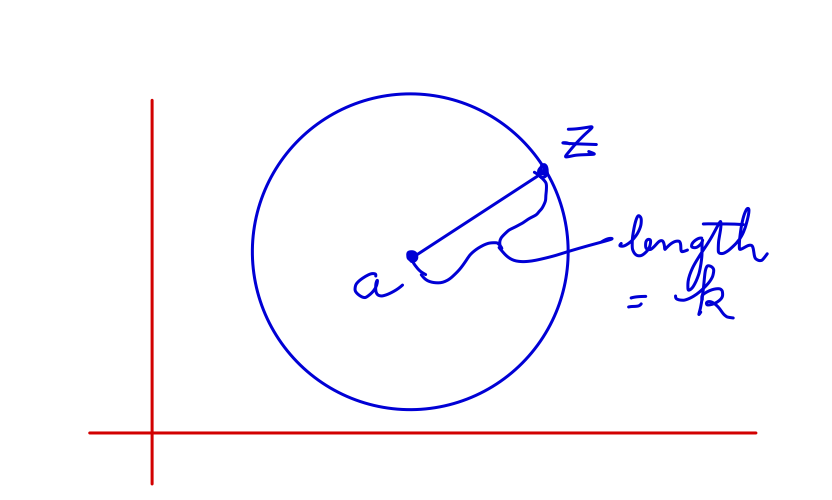
\includegraphics[width=.4\textwidth]{Q2circ.jpeg} \qquad  \qquad 
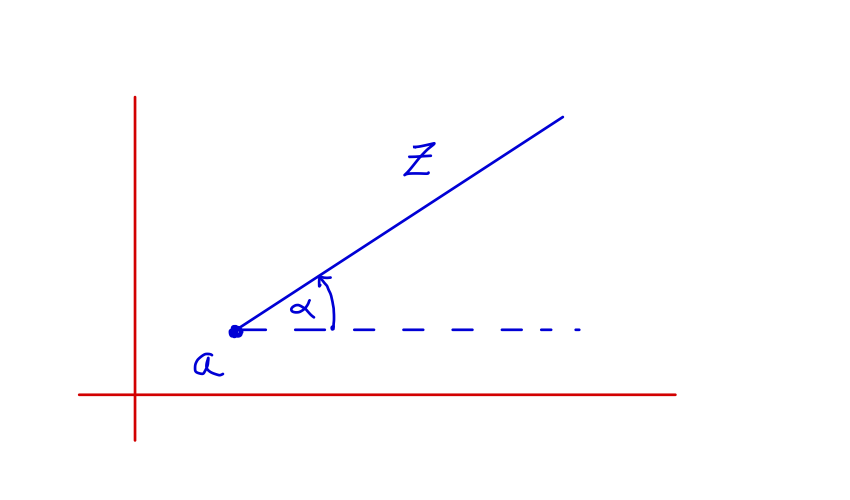
\includegraphics[width=.4\textwidth]{Q2line.jpeg} 
\end{center}
(a) The first sketch is the circle represented by $ |z-a| = k $.\\
(b) The second sketch is the line segment given by $ \arg(z-a) = \alpha $. 

\begin{center}
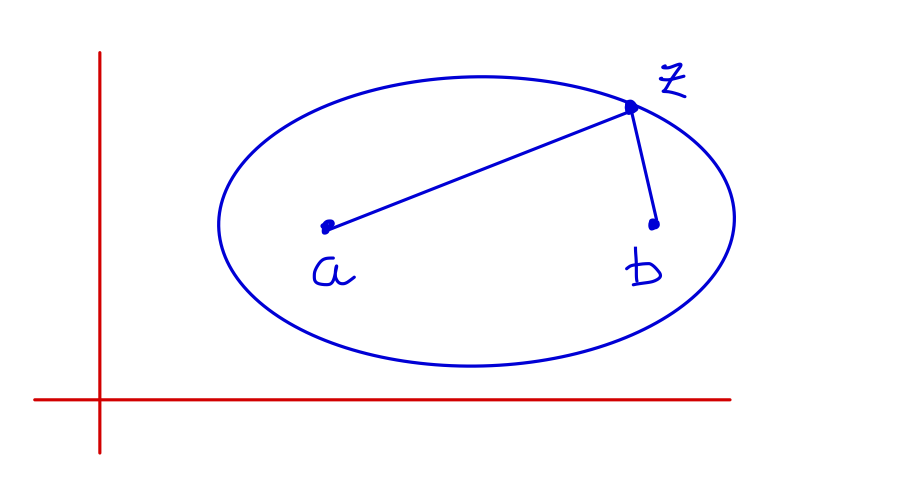
\includegraphics[width=.4\textwidth]{Q2ellipse.jpeg}  
 \end{center}
(c) The third sketch is the ellipse given by  $ |z-a| + |z-b| = c $, where the line segments connecting $ z $ to $ a $ and $ b $ have lengths $ |z-a| $ and $ |z-b | $ respectively, and sum to $ c $.

\bigskip
\noindent \phantom{2. } (ii)  Let $ z = r e^{i\theta} $ in polar form. By assumption, $ r \neq 0 $. 

\bigskip
(a)  We have
\[
u = z + \frac{|z|^2}{z}  = re^{i\theta} + \frac{r^2}{re^{i\theta}} = r\left(e^{i\theta} + e^{-i\theta}\right) = 2r\cos\theta ,
\]
which in particular is real.

\bigskip
(b)  By assumption, $ z $ has real part not zero, or equivalently $ z $ is not pure imaginary, or equivalently in polar form $ \theta \neq \frac{\pi}{2}, \frac{3\pi}{2} $.  
Then
\begin{align*} 
v = \frac{|z|-iz}{|z|+ iz} &= \frac{r-ir e^{i\theta}}{r+ir e^{i\theta}}   =  \frac{1-i e^{i\theta}}{1+i e^{i\theta}}   
	 =  \frac{1-i e^{i\theta}}{1+i e^{i\theta}} \times \frac{1-i e^{-i\theta}}{1-i e^{-i\theta}}  
			 = \frac{1-i e^{-i\theta} -i e^{i\theta} -1}{1-i e^{-i\theta} +i e^{i\theta} +-1} \\
	 &= \frac{-2i\cos \theta}{2-2\sin \theta} = -i\frac{\cos \theta}{1-\sin  \theta}
			=  -i\frac{\cos \theta}{1-\sin  \theta} \times \frac{1 + \sin \theta}{1 + \sin \theta}\\
			 	&=  -i\frac{\cos\theta(1 + \sin \theta)}{  \cos^2 \theta}
				= -i\frac{1 + \sin \theta}{\cos \theta} = -i(\sec \theta + \tan \theta).
\end{align*} 
The assumptions on $ z $ were used to ensure the denominator in the definition of $ v $ is non-zero, and the denominators $ 1-ie^{-i\theta} $ and $ 1+\sin\theta $ introduced in the first and second lines above are also non-zero.
\end{proof} 

\bigskip

\paragraph{Tips \& Tricks} In part (ii)   first write $ z $ in the form $ re^{i\theta} $.  Then part (ii)(a) is easy.

\medskip
For part (ii)(b), in the first line for the calculation of $ v $, the term   $ (1-i e^{-i\theta})$ in the introduced factor $ 1 = (1-i e^{-i\theta})/(1-i e^{-i\theta}) $ is just the complex conjugate of $  1+i e^{i\theta}$. In this way the new denominator of $ v $ is real. (So this is a good move)

In the second line of the calculation the term $ 1+ \sin \theta $, in the new factor $ 1 = (1+\sin \theta)/(1+\sin \theta) $, has the property that when multiplied by $ 1-\sin\theta $ the result is $ \cos^2 \theta $ (which is the second good move).


%%%%%%%%%%%%%%%%%%%%%%%%%%%%%%%%%%%%%%%%%%%%%%%%%%%%%%%
%%%%%%%%%%%%%%%%%%%%%%%%%%%%%%%%%%%%%%%%%%%%%%%%%%%%%%%%
\newpage
\section*{Question 3}

\paragraph{Part 1} $ F $ is the point $ (ae,0) $ and $ d $ is the line $ x =a/e $ ($ e> 1 $).  $ M $ is the foot of the perpendicular from a variable point $ P $ to $ d $, and $ P $ moves so that 
\[
FP^2 = e^2 PM^2 .
\]
Find the equation of the locus.

Draw a sketch showing clearly the principal axes of the curve, the foci, the directrices and the asymptotes, marking on each of them its equation or coordinates.

Express $ e $ in terms of $ \alpha $, the angle between the asymptotes. 

\paragraph{Part 2}
A line, parallel to one asymptote, is drawn through a focus $ F $ of a hyperbola.  It meets the hyperbola in $ H $, the directrix corresponding to $ F $ in $ D   $, the other asymptote in $ K $ and the conjugate axis in $ R $.  Prove that
\begin{align*}
FH &= HD, \\  FK &= KR.
\end{align*}  

\bigskip


\begin{proof}[Solution] \mbox{}


\paragraph{Part 1}\mbox{}
\begin{figure}[!hbtp]
\begin{center}
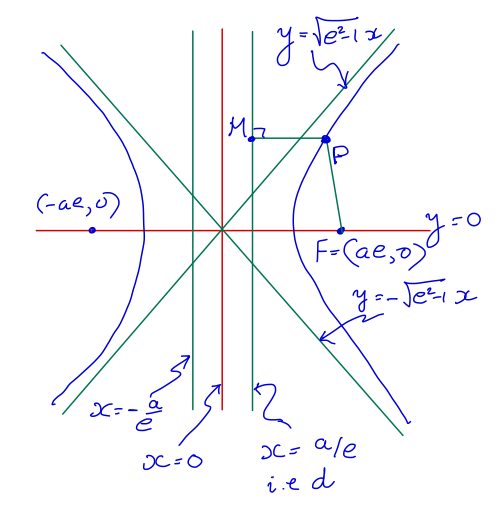
\includegraphics[width=.45\textwidth]{Q3.jpeg} 
\caption{Hyperbola with focus $ F $ and directrix $ d $, traced out by $ P $ moving so $ FP^2 = e^2 PM^2 $.}
\label{F3}
\end{center}
\end{figure}

See Figure~\ref{F3}.
Let $ P $ be the point $ (x,y) $.  Then $ M= (a/e, y) $.  Since $ FP^2 = e^2 PM^2$, it follows that 
\begin{align}
(x-ae)^2 + y^2 &= e^2 (x-a/e)^2 = (ex-a)^2 \notag \\
\therefore \quad a^2  (e^2 - 1 ) &= x^2(e^2-1 ) - y^2  \notag \\
\therefore \quad \frac{x^2}{a^2} - \frac{y^2}{a^2(e^2-1)} &= 1. \label{gf}
\end{align} 
The last equation is the equation of the locus.  It is in the standard form $ \dfrac{x^2}{a^2} - \dfrac{y^2}{b^2} = 1 $ for an hyperbola, with $ b= a\sqrt{e^2 -1} $.

It follows from standard formulae for an ellipse that 
\begin{itemize} [nosep]
\item the principal axes are $ y=0 $ and $ x=0 $, 
\item the foci are $ \pm \left(   \left(a^2 + b^2\right)^{1/2}, 0 \right) = \pm ( ae , 0 ) $, 
\item the directices are  
$ x = \pm\dfrac{a^2}{\sqrt{a^2 + b^2 } }$, i.e.\ $ x = \pm a/e $ (i.e.\ the line $ d $ and its mirror image in the $ y $-axis), 
\item and the asymptotes are $ y = \pm \dfrac{b}{a}\, x$, i.e.\ $ y = \pm \sqrt{e^2-1}\, x $.
\end{itemize} 
 
 If $ \alpha $ is the angle between the asymptotes then $ \tan (\alpha /2) = \sqrt{e^2 -1} $ and so $ \alpha = 2 \arctan \sqrt{e^2-1} $.

We can also simplify this as follows:
 \begin{align*}
 \tan^2 \frac{\alpha  }{2} &= e^2 -1 \\ 
 \therefore \quad \sin^2 \frac{\alpha  }{2} &= e^2 \cos^2\frac{ \alpha }{2} -    \cos^2\frac{ \alpha }{2} \\
 \therefore \quad 1 &= e^2 \cos^2\frac{ \alpha }{2} \\
\therefore \quad \cos \frac{ \alpha }{2} &= e^{-1}\\
 \therefore \quad \alpha &= 2 \arccos{(e^{-1})}.
 \end{align*} 


\bigskip
\paragraph{Part 2} \mbox{}

\begin{figure}[!hbtp]
\begin{center}
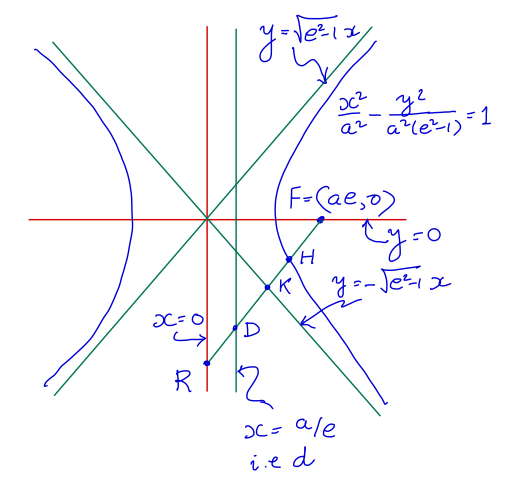
\includegraphics[width=.45\textwidth]{Q3-2.jpeg} 
\caption{$ FH = HD $, $ FK = KR $.}
\label{F3-2}
\end{center}
\end{figure}


See Figure~\ref{F3-2}. We can take the hyperbola to be the same as that in Part 1, since the most general hyperbola can be represented in the standard form $ \dfrac{x^2}{a^2} - \dfrac{y^2}{b^2} = 1 $,   and~\eqref{gf}  is in this form if we take $ e = \sqrt{1 + \frac{b^2}{a^2}} $.

 The equation of the line through $ F $ and parallel to   the asymptote $ y = \sqrt{e^2-1}\, x $ is
\[ 
y = \sqrt{e^2 -1}\, (x-ae) 
\]
since this has the required slope and passes through $ F $. (If we took the second asymptote the following argument would be similar.  But it is also clear that it is sufficient to just do one case, as the other in essence follows geometrically be reflecting everything in the $ x$-axis.)


 In order to prove $ FH  = HD$ and $  FK  = KR$, since these are parallel segments,   it is sufficient to prove that the corresponding projections onto the $ x $-axis are equal.
  We write $ FH_x $ etc. for these projections, and similarly write $ F_x $, $ H_ x $ etc.\ for the $ x $-coordinates of $ F $, $ H $ etc.
 
 Then
 \begin{itemize} [nosep]
 \item $ F_x = ae $.

 \item At $ H $, $ y = \sqrt{e^2 -1}\, (x-ae) $ and $ x^2- y^2/(e^2-1) = a^2 $.  Hence $ x^2 - (x-ae)^2 = a^2 $, therefore $ 2xae = a^2(1+e^2) $ and so $ x = a/(2e) + ae/2 $. That is
 \[
 H_x = \frac{a}{2e} + \frac{ae}{2} .
 \]
  
 \item At $ K $, $ y = \sqrt{e^2 -1}(x-ae) $ and $ y = -\sqrt{e^2 -1}\, x $,   so $ x =ae/2 $. That is
 \[
 K_x = \frac{ae}{2}.
 \]
 
 \item Clearly,
 \[
 D_x = \frac{a}{e}, \qquad R_x = 0 .
 \]
 \end{itemize}
 
 
 It follows that 
 \begin{align*}
 FH_x &= F_x - H_x = \frac{a}{2e} - \frac{ae}{2}, \\
 HD_x &= H_x - D_x =  \frac{a}{2e} - \frac{ae}{2}, \\
 FK_x &= F_x - K_x = \frac{ae}{2},\\
 KR_x &= K_x - R_x = \frac{ae}{2}.
\end{align*} 
This proves the required equalities.
\end{proof} 
 
 
 
 %%%%%%%%%%%%%%%%%%%%%%%%%%%%%%%%%%%%%%%%%%%%%%%%%%%%%%%
%%%%%%%%%%%%%%%%%%%%%%%%%%%%%%%%%%%%%%%%%%%%%%%%%%%%%%%%
\newpage
\section*{Question 4}

Express $ x^n - 1 $ as a product of real linear or quadratic factors, distinguishing the cases $ n $ odd and $ n $ even.

Thence or otherwise prove that
\[
\sin\frac{\pi}{n} \sin\frac{2\pi}{n} \ldots \sin \left(\frac{n-1}{2n} \pi \right) = \sqrt{\frac{n}{2^{n-1}}}
\]
when $ n $ is odd, and find the corresponding result when $ n $ is even.

\bigskip
\begin{proof} \mbox{}

First assume $ n $ is odd.  Then the solutions of $ x^n = 1 $ can be written in the form\footnote{The solutions are uniformly distributed around the unit circle in the complex plane.  They are written here in complex conjugate pairs, apart from the solution $ x=1 $.} 
\[
x=1, \qquad x = e^{\pm   \frac{2\pi i }{n}j} \quad \text{for } j =1,\dots, \frac{n-1}{2}.
\]
Hence 
\begin{align}
x^n - 1 &= (x-1)   \prod_{j=1}^{\frac{n-1}{2}} \left(x- e^{  \frac{2\pi i }{n}j} \right) \left(x- e^{-  \frac{2\pi i }{n}j} \right) \notag \\
	&= (x-1)  \prod_{j=1}^{\frac{n-1}{2}} \left( x^2 - 2x\cos\left(\frac{2\pi j}{n}   \right) +1 \right). \label{fac1}
\end{align}
This is a product of real linear and quadratic factors, as required.

\bigskip
 
Dividing both sides by $ x-1 $ it follows that for $ x\neq 1  $
\begin{equation} \label{tricky} 
1+x+x^2 + \dots + x^{n-1} = \prod_{j=1}^{\frac{n-1}{2}} \left( x^2 - 2x\cos\left(\frac{2\pi j}{n}  \right) +1 \right).
\end{equation} 

Since both sides are polynomials in $ x $ the limit as $ x \to 1 $ of both sides are equal, and so
\[
n  = \prod_{j=1}^{\frac{n-1}{2}} \left(  2 - 2 \cos\left(\frac{2\pi j}{n}   \right)   \right)  
	 =  \prod_{j=1}^{\frac{n-1}{2}}  4 \sin^2 \left(\frac{ \pi j}{n} \right)    
	 = 2^{n-1}  \prod_{j=1}^{\frac{n-1}{2}}    \sin^2 \left(\frac{ \pi j}{n} \right) ,
\]
using $ \cos (2\theta) = 1 - 2\sin^2 \theta $.
Taking the square root of each side and noting each of the  sine   terms is positive,
\begin{equation} \label{fac2} 
\prod_{j=1}^{\frac{n-1}{2}}    \sin  \left(\frac{ \pi j}{n} \right) = \sqrt{\frac{n}{2^{n-1}}},
\end{equation} 
as required.

\bigskip
If $ n $ is even, then the solutions of $ x^n = 1 $ can be written in the form 
\[
x=\pm 1, \qquad x = e^{\pm   \frac{2\pi i }{n}j} \quad \text{for } j =1,\dots, \frac{n}{2}-1.
\]
Hence 
\begin{align}
x^n - 1 &= (x-1)(x+1)   \prod_{j=1}^{\frac{n}{2}-1} \left(x- e^{  \frac{2\pi i }{n}j} \right) \left(x- e^{-  \frac{2\pi i }{n}j} \right) \notag\\
	&= (x-1)(x+1)  \prod_{j=1}^{\frac{n}{2}-1} \left( x^2 - 2x\cos\left(\frac{2\pi j}{n}   \right) +1 \right).
\end{align}
This is again a product of real linear and quadratic factors, as required.

\bigskip
Dividing both sides by $ x-1 $ it follows that for $ x\neq 1  $
\[
1+x+x^2 + \dots + x^{n-1} = (x+1)\prod_{j=1}^{\frac{n}{2}-1} \left( x^2 - 2x\cos\left(\frac{2\pi j}{n}  \right) +1 \right).
\]
Once again taking the limit as $ x\to 1 $, 
\[
n  = 2\prod_{j=1}^{\frac{n}{2}=1} \left(  2 - 2 \cos\left(\frac{2\pi j}{n}   \right)   \right)  
	 = 2 \prod_{j=1}^{\frac{n}{2}-1}  4 \sin^2 \left(\frac{ \pi j}{n} \right)    
	 = 2 \times 2^{n-2}  \prod_{j=1}^{\frac{n}{2}-1}    \sin^2 \left(\frac{ \pi j}{n} \right) 
	 =   2^{n-1}  \prod_{j=1}^{\frac{n}{2}-1}    \sin^2 \left(\frac{ \pi j}{n} \right) .
\]
Again taking the square root of both sides,
\begin{equation} \label{} 
\prod_{j=1}^{\frac{n}{2}-1}    \sin  \left(\frac{ \pi j}{n} \right) = \sqrt{\frac{n}{2^{n-1}}},
\end{equation} 
as required.
\end{proof} 



\bigskip

\paragraph{Tips \& Tricks} Obtaining the  factorisation in~\eqref{fac1} is not that difficult, once you know how to pair conjugate  roots to get real quadratic factors.  
More precisely, if $ x=w $ and $ x= \overline{w} $ are both solutions of $ x^n = 1 $, the $ x-w $ and $ x - \overline{w} $ are both factors and hence so is 
\[ (x-w)(x-\overline{w} ) = x^2 - 2 x \Re(w) + |w|^2, \]   
which is real quadratic and where $ \Re $ means ``the real part of''.

But the other problem in getting to~\eqref{fac2} from~\eqref{fac1} is that the angles in~\eqref{fac1} have increments $ 2\pi/n $, whereas in~\eqref{fac2} the incrments are $ \pi/n $.  This leads one to considering the formula $ \cos (2\theta) = 1 - 2\sin^2 \theta $, which indicates the approach to take.  

The final twist is that one really needs $ x=1 $ in~\eqref{tricky}, whereas it was derived under the assumption $ x \neq 1 $. The more general fact that has been used is that if $ f(x) = (x-a)\, g(x) $ for $  x=a $ and all   $ x $ near $ a $, then $ f'(a) = g(a) $. (Assuming $ g $ is continuous at $ a $.  \emph{Exercise}.)




 %%%%%%%%%%%%%%%%%%%%%%%%%%%%%%%%%%%%%%%%%%%%%%%%%%%%%%%
%%%%%%%%%%%%%%%%%%%%%%%%%%%%%%%%%%%%%%%%%%%%%%%%%%%%%%%%
\newpage
\section*{Question 5}

Draw a sketch to show the relation between the point  $ (a\cos\phi, b\sin\phi ) $ on the ellipse $ x^2/a^2 + y^2/b^2 = 1 $ and the corresponding point on the auxiliary circle.\footnote{The auxiliary circle for an ellipse is the circle whose diameter is the major axis of the ellipse.}

Write down the equation of the circle on which the points $ (x_1,y_1) $, $ (x_2,y_2) $ are the extemities of a diameter.

$ P $ is a variable point on an ellipse of which $ F $ is one focus.  Prove the circle on $ PF $ as diameter touches the auxiliary circle of the ellipse.


\bigskip



\begin{proof}[Solution] \mbox{}

\bigskip

Without loss of generality we take $ a> b $.

\noindent \textbf{1.} \mbox{}

\begin{figure}[!hbtp]
\begin{center}
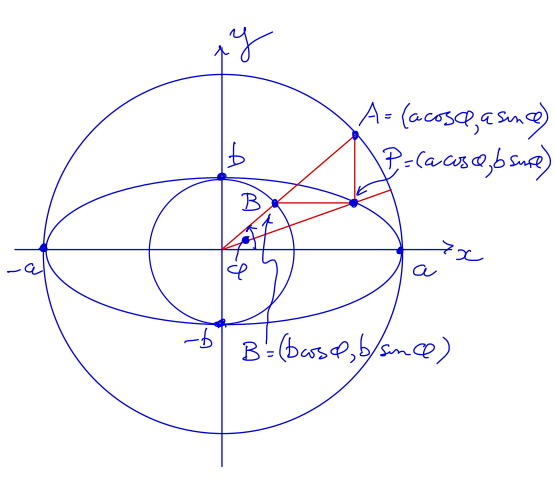
\includegraphics[width=.45\textwidth]{Q5.jpeg} 
\caption{The larger circle is the auxiliary circle for the ellipse.}
\label{F5}
\end{center}
\end{figure}

  See Figure~\ref{F5}.  The question is a little ambiguous, but the point corresponding to $ P $ on the auxiliary circle (outer) circle $ O $ is usually taken to be $ A =   (a\cos\phi, a \sin \phi) $.  (The point corresponding to P on the inner circle is $ B = (b\cos\phi, b \sin \phi)$.)  

\bigskip  \noindent \textbf{2.} \quad 
The equation of the circle on which the points $ (x_1,y_1) $, $ (x_2,y_2) $ are the extemities of a diameter is
\[
(x-x_1)^2 + (y-y_1)^2 + (x-x_2)^2 + (y-y_2)^2 = (x_1-x_2)^2 + (y_1-y_2)^2,
\]
which simplifies to
\begin{equation} \label{eqc}
x^2 + y^2 -x(x_1 + x_2) -y(y_1 + y_2) + (x_1x_2 +  y_1 y_2) = 0.
\end{equation} 

\bigskip

\noindent \textbf{3} \quad 
\begin{figure}[!hbtp]
\begin{center}
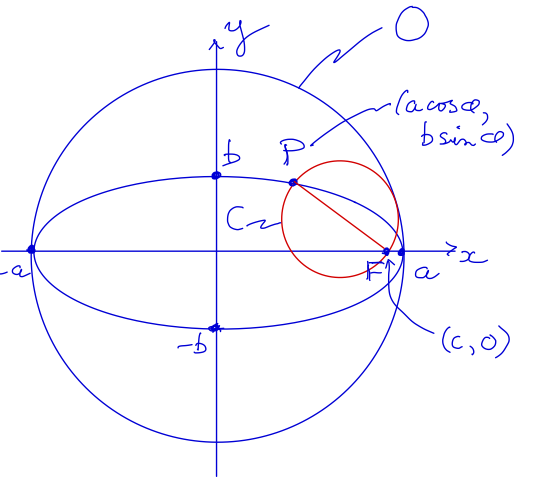
\includegraphics[width=.5\textwidth]{Q5-2.jpeg} 
\caption{Ellipse with auxiliary circle $ O $.  The   circle $ C $ with diameter $ PF $ touches $ O $.}
\label{F5-2}
\end{center}
\end{figure}
See Figure~\ref{F5-2}. The focus $ F $ has coordinates $ (\pm c,0) $ where 
\begin{equation} \label{prc}
c>0, \quad c^2 = a^2 - b^2 .
\end{equation}
  Without loss of generality because of symmetry, we take $ F = (c,0)$.

The point $ P $ on the ellipse has coordinates $ (a\cos\phi, b\sin\phi ) $ for some $ \phi \in [0,2\pi)$.
Fix $ \phi $. From \eqref{eqc}, the equation of the circle $ C $ on $ PF $ as diameter is
\begin{equation} \label{oac} 
x^2 + y^2 - x (a \cos\phi +c) - y\, b \sin\phi + a\, c\cos\phi = 0.
\end{equation} 
In order to prove the circle $ C $ on $ PF $ as diameter touches the auxiliary circle $ O $ of the ellipse, we will show that   every point $ (x,y) \in O $   satisfies 
\begin{equation} \label{boc} 
 x^2 + y^2 - x (a \cos\phi +c) - y\, b \sin\phi + a\, c\cos\phi \geq  0,
\end{equation} 
and that some point $ (x,y) \in O $   satisfies~\eqref{oac}. 

Take an arbitrary point $ (x,y) = (a\cos\theta , a \sin\theta ) \in O $, and substituting into the left side of~\eqref{boc} we want to show 
\begin{equation} \label{sthmin} 
a\big( a -   \cos \theta ( a \cos\phi +c) -  b \sin\theta \sin\phi + c \cos\phi \big) \geq 0 
\end{equation} 
for all $ \theta$, and show that equality holds for some $ \theta $.


\medskip
Using the trigonometric identities 
\begin{equation} \label{tids}
t = \tan \frac{\theta}{2}, \quad \sin\theta = \frac{2t}{1+t^2} , \quad \cos\theta = \frac{1-t^2 }{1+t^2 } , \quad \tan\theta = \frac{2t}{1-t^2 } ,
\end{equation} 
we want to show  for all $ t $ that 
\begin{equation} \label{} 
a - a  \frac{1-t^2 }{1+t^2 }\cos\phi - b \frac{2t}{1+t^2}\sin\phi + c \left( \cos\phi - \frac{1-t^2 }{1+t^2 }\right) \geq 0 ,
\end{equation} 
and that equality holds for some $ t $.

Multiplying  through by the positive term $ 1+t^2 $ we obtain the following quadratic in $ t  $:
\begin{align}
&a(1+t^2) -a(1-t^2)\cos\phi -2bt\sin\phi + c(1+t^2)\cos\phi - c(1-t^2)  \notag\\
&= t^2(a+a\cos\phi + c \cos\phi +c) -2bt \sin\phi + (a-a\cos\phi +c\cos\phi - c) \notag\\
&= t^2(a+c)(1+\cos\phi) -2bt \sin\phi  + (a-c)(1-\cos\phi).   \label{mqu}
\end{align}
Assuming initially that $ \phi \neq \pi$, it follows that the coefficient of $ t^2 $ is $ > 0 $.  The discriminant of the quadratic is
\begin{equation} \label{} 
4 \left( b^2\sin^2 \phi -(a^2-c^2)(1-\cos^2 \phi) \right) = 4 (b^2-a^2 + c^2 )\sin^2 \phi =0,
\end{equation} 
using~\eqref{prc}.

Since the quadratic~\eqref{mqu} has zero discriminant and positive leading term, it is always $ \geq 0 $, and takes the minimum value $ 0 $. Moreover, this minimum value occurs at 
\begin{equation} \label{tmin}
t = \frac{2b\sin\phi}{ 2(a+c)(1+\cos\phi) } = \frac{ b\sin\phi}{  (a+c)(1+\cos\phi) }.
\end{equation} 

This answers the question if $ \phi \neq \pi $, since it follows that the circle $ C $ lies inside the auxiliary circle $ O $ and meets the auxiliary circle  when $ t $ is as in~\eqref{tmin}.  Moreover, $ C $ and the auxiliarly circle  must touch tangentially from geometric considerations.  This also follows from the fact that the derivative of the quadratic~\eqref{mqu} at  the minimum is zero.

Finally, if $ \phi =\pi $ then $ P = (-\pi, 0) $, and from the previous diagram it is clear in this case that $ C $ lies inside the auxiliary circle and the two circles touch at $ P $.
\end{proof}

\bigskip

\paragraph{Tips \& Tricks} Once we have reached~\eqref{sthmin}, it is reasonable to think about minimising a quadratic, and to guess that one possibility might be to use the half angle identities in~\eqref{tids}. Fortunately, with a little care, this does work.


\bigskip
\paragraph{Addendum} \mbox{}

\begin{figure}[!hbtp]
\begin{center}
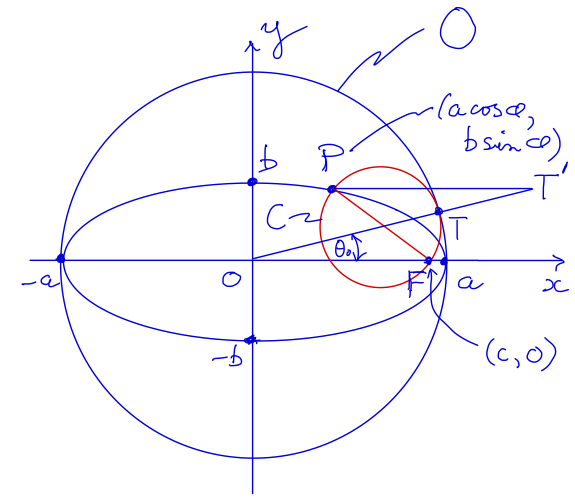
\includegraphics[width=.45\textwidth]{Q5-3.jpeg} 
\caption{Geometric construction of the touching point $ T $ of the red circle and the auxiliary circle.  $ PT' $ is parallel to and has equal length to $ OF $.}
\label{F5-3}
\end{center}
\end{figure}

 From~\eqref{tids} and~\eqref{tmin}, the value of $  \theta_0$ for the point $ T = ( a \cos \theta_0, a \sin \theta_0) $ at which $ C $ touches the auxiliary circle, satisfies
\begin{equation} \label{stmin}
 \tan \theta_0 = \frac{2t}{1-t^2 },
 \end{equation}
 where $ t $ is as in~\eqref{tmin}. 

We calculate 
\begin{align*}
1-t^2 &= 1 - \frac{b^2 \sin^2\phi}{(a+c)^2(1+\cos \phi)^2} \\
&= \frac{(a+c)^2(1+\cos \phi)^2 - (a^2 -c^2)(1-\cos^2\phi)} { (a+c)^2(1+\cos \phi)^2} \qquad \text{(from \eqref{prc})}\\
&= \frac {(a+c)(1+\cos\phi) - (a-c)(1-\cos \phi)}  { (a+c) (1+\cos\phi) }\\
&= \frac {2(a \cos\phi +c  ) } { (a+c) (1+\cos\phi) }.
\end{align*} 
From this, \eqref{tmin} and \eqref{stmin} it follows that 
\[
\tan \theta_0 = \frac{b\sin\phi}{a\cos\phi+ c}, \quad \theta_0 = \arctan  \frac{b\sin\phi}{a\cos\phi+ c}  .
\]

Looking at Figure~\ref{F5-3}, it follows that the point $ T $ can be found as follows. Draw a line parallel to the $ x $-axis through $ P $ and move taway from the $ y $-axis  by a distance equal to the focal length $ c $. Call this point $ T' $ and  draw  a straight line from the origin  through  $ T' $.  Then $ T $ is the intersection point of this line with the auxiliary circle. (\emph{Why?})


%%%%%%%%%%%%%%%%%%%%%%%%%%%%%%%%%%%%%%%%%%%%%%%%%%%%%%%
%%%%%%%%%%%%%%%%%%%%%%%%%%%%%%%%%%%%%%%%%%%%%%%%%%%%%%%%
\newpage
\section*{Question 6}

Prove that the feet of the four normals to the ellipse, $ E=0 $, where $ E \equiv x^2/a^2  +   y^2/b^2 -1 $, from the point $ (x_1,y_1) $ are the intersections of $ E=0 $ with the rectangular hyperbola $ H_1 = 0 $, where
\[
H_1 \equiv \left( \frac{1}{b^2} - \frac{1}{a^2} \right) xy + \frac{y_1}{a^2}\, x - \frac{x_1}{b^2}\, y .
\]

Give a reason why, if $ \lambda H_1 + E = 0 $ represents a line pair\footnote{This means that $  \lambda H_1 + E   $ can be written as a product of two linear factors.  Note that in this case,  if both $  H_1 =0 $ and $  E  =0 $ then  at least one of the two linear factors equals zero.}, then this line pair is one of the three which join pairs of the feet of the four normals.

The join of the feet of two of these four normals is the line
\[
\frac{l x}{a} + \frac{my}{b} + 1 = 0 ;
\]
prove that the join of the other two feet is 
\[
\frac{x}{la}m+ \frac{y}{mb} - 1 = 0.
\]

Find the values of $ x_1, y_1 $ in terms of $ l,m $.


\bigskip
\begin{proof}[Solution] \mbox{}
\begin{figure}[!hbtp]
\begin{center}
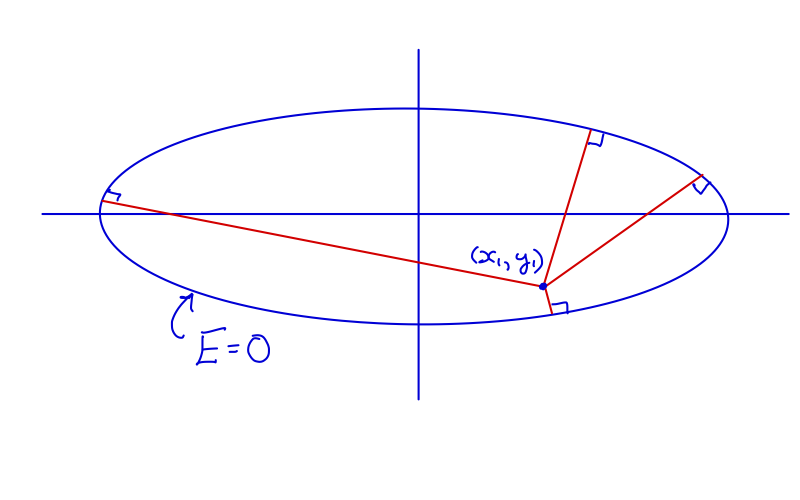
\includegraphics[width=.55\textwidth]{Q6ell.jpeg} 
\caption{Ellipse  and the four normals from a point $ (x_1,y_1) $.}
\label{F6-1}
\end{center}
\end{figure}

\noindent \textbf{1} \quad The normal to $ E =  0 $ at  $ (x,y) $, which  is the direction of maximum increase in $ E = E(x,y) $ at $ (x,y) $,   is given by 
\[ 
\left( \frac{\partial E}{\partial x}, \ \frac{\partial E}{\partial y} \right) =  \left( \frac{2x}{a^2}, \frac{2y}{b^2} \right)
=  2\left( \frac{x}{a^2}, \frac{y}{b^2} \right).
\]
So $ P =(x, y) $ is the foot of a normal from $(x_1,y_1) $ to $ E=0 $ if and only if
\begin{itemize}
\item [(i)] $ \dfrac{x^2}{a^2} + \dfrac{y^2}{b^2}  -1 = 0 $, and
\item [(ii)]  $ \dfrac{x-x_1}{x/a^2 } = \dfrac{y-y_1}{y/b^2 } $.
\end{itemize} 
We can rewrite (ii) as 
\[
 \left(\frac{1}{b^2} - \frac{1}{a^2} \right) xy + \frac{y_1}{a^2}\, x - \frac{x_1}{b^2}\, y = 0 .
 \]
Hence  the feet of the four normals to   $ E=0 $ from $ (x_1,y_1) $ are the intersections of $ E=0 $ with  $ H_1 = 0 $.

\bigskip 
\noindent \textbf{2} \quad 
Suppose $   \lambda H_1 + E = 0 $ represents the line pair $ a_1 x + b_1y + c_1 =0 $ and $ a_2 x + b_2 y + c_2 =0 $.  This means that for some $ a_1,b_1 ,c_1 $ and $ a_2,b_2 ,c_2 $, and for all $ x,y $,
\begin{equation} \label{lp} 
 \lambda H_1 + E \equiv ( a_1 x + b_1y + c_1 ) ( a_2 x + b_2 y + c_2).
\end{equation} 


At each of the four points $ P =P(x,y) $ which are the feet of the four normals, one   has $ E=0 $ and $ H_1 = 0 $ and so either $  a_1 x + b_1y + c_1  = 0 $ or $ a_2 x + b_2y + c_2  = 0$.  Since no three points on $ E = 0 $ are in a straight line, two of the feet must satisfy $  a_1 x + b_1y + c_1  = 0 $ and the other two satisfy $  a_2 x + b_2y + c_2  = 0 $. 

In other words, the line pair is one of the three which join pairs of the feet of the four normals.

\bigskip 
\noindent \textbf{3} \quad 
It is given that  the join of the feet of two of these four normals is the line
\[
\frac{l x}{a} + \frac{my}{b} + 1 = 0 .
\]
(Note that any line can be written in this form.)

It follows from~\eqref{lp} that   the    join of the other two feet can be written in the form  $ \alpha x + \beta y + \gamma = 0 $, where
\begin{equation} \label{6me} 
\lambda \left(  \left( \frac{1}{b^2} - \frac{1}{a^2} \right) xy + \frac{y_1}{a^2}\, x - \frac{x_1}{b^2}\, y \right)
+  \dfrac{x^2}{a^2} + \dfrac{y^2}{b^2}  -1  = 
\left( \frac{l x}{a} + \frac{my}{b} + 1\right) \left( \alpha  x + \beta  y + \gamma \right)
\end{equation} 
for all $ x ,  y $.

Equating the coefficients of $ x^2, y^2 $ and the constant terms, gives rspectively,
\begin{equation} \label{6ine}
  \alpha = \frac{1}{la},\quad  \beta = \frac{1}{mb},  \quad      \gamma = -1. 
  \end{equation}
 That is, the join of the other two feet is
\begin{equation} \label{}
\frac{x}{la} + \frac{y}{mb} -1 = 0.
\end{equation} 

\bigskip 
\noindent \textbf{4} \quad From~\eqref{6me}, using \eqref{6ine} and equating the coefficients of $ xy $,
\begin{align} 
\lambda \left( \frac{1}{b^2} - \frac{1}{a^2} \right) &=\frac{l \beta }{a} + \frac{m \alpha }{b} 
	= \frac{l}{abm} + \frac{m}{abl} = \frac{l^2 + m^2}{ablm} \notag\\
\therefore \quad \lambda &= \frac{ab(l^2 + m^2)}{(a^2 - b^ 2)lm}. \label{6eqlam}
\end{align} 
 Again from \eqref{6me}, equating the coefficients of $ x $ and of $ y $ and using~\eqref{6ine} and~\eqref{6eqlam}, gives respectively
 \begin{equation} \label{6xy1}
 \begin{aligned}
 y_1 &= \frac{ a^2 \alpha}{ \lambda } =  a^2\, \frac{1}{ l a}\  \frac{(a^2 - b^2)lm }{ab\,  ( l^2 + m^2) }  
 	=  \frac{(a^2 - b^2) m }{ b\,  ( l^2 + m^2) },\\
x_1 &=  -\frac{ b^2 \beta }{ \lambda } =  -b^2\, \frac{1}{ mb}\  \frac{(a^2 - b^2)lm }{ab\,  ( l^2 + m^2) }  
 	=  -\frac{(a^2 - b^2) l }{ a\,  ( l^2 + m^2) }.
 \end{aligned}
 \end{equation} 
 \end{proof} 


\bigskip

\paragraph{Tips \& Tricks} 
\begin{enumerate}[nosep]
\item The first point is that the normal to $ E=0 $ points in the direction of maximum increase ot the quantity $ E $.  Ths is a general and important fact.

\item The idea of a quadratic in two variables (here $ \lambda H_1 + E $ for some $ \lambda $) being factorisable into two linear factors is interesting and used in the subject of algebraic geometry. 

\item Note how \eqref{6eqlam} and \eqref{6xy1}  are proved by equating coefficients.
\end{enumerate} 





%%%%%%%%%%%%%%%%%%%%%%%%%%%%%%%%%%%%%%%%%%%%%%%%%%%%%%%
%%%%%%%%%%%%%%%%%%%%%%%%%%%%%%%%%%%%%%%%%%%%%%%%%%%%%%%%
\newpage
\section*{Question 7}

Sketch the graph of the function 
\[
 x = \tan y 
\] 
and indicate how a range of principal values of the inverse tangent should be chosen.
Denoting the principal value of he inverse tangent by $ \tan^{-1} x $, give a formula for the general value of the inverse tangent.

If a sequence is defined by 
\begin{equation} \label{undef} 
\begin{aligned}
u_0 &=1 \\
u_{n+1} &= \frac{2^{n+1} u_n +1 }{2^{n+1} - u_n }
\end{aligned}
\end{equation} 
show that 
\begin{equation} \label{7wf} 
 \lim_{n\to\infty } \tan^{-1} u_n = \dfrac{\pi}{4} + \sum_1^\infty \tan^{-1} \dfrac{1}{2^n}.
\end{equation} 

Using the tables compute the value of this limit to two significant figures.

  
\bigskip
\paragraph{\color{red}Spoiler}  The limit \eqref{7wf} is wrong, see~\eqref{7wff}.


\bigskip
\begin{proof}[Solution] \mbox{}

\begin{figure}[!hbtp]
\begin{center}
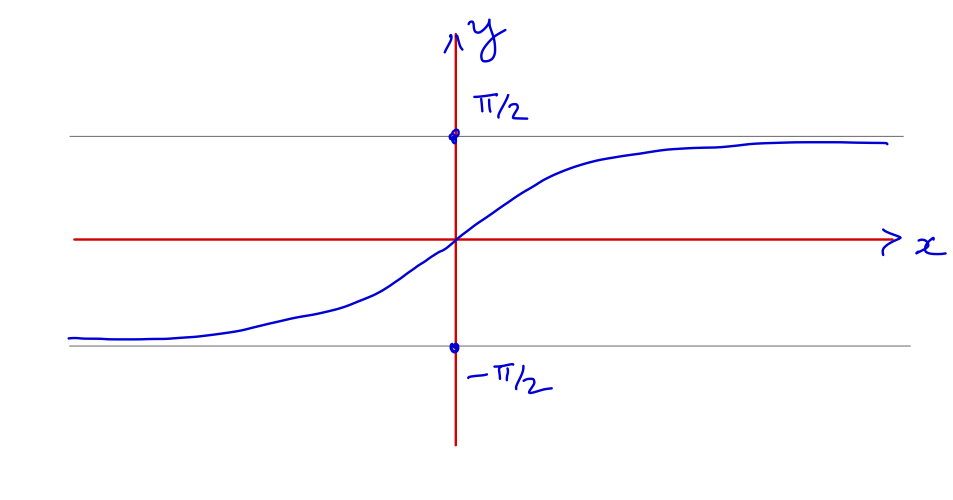
\includegraphics[width=.55\textwidth]{Q7.jpeg} 
\caption{Graph of $ y= \tan^{-1} x $ (i.e.\ of $ x =\tan y $ for $ y \in (-\pi/2, \pi/2 ) $)}
\end{center}
\end{figure}

%\begin{figure}[!hbtp]
%\begin{center}
%%\includegraphics[width=.5\textwidth]{image7.jpeg} 
%\includegraphics[width=.3\textwidth]{states+-.png} 
%\caption{A section of $ \mathbb{C} ^2 $.  (from~\cite{Vazirani2})  }  
%\end{center}
%\end{figure}


\noindent \textbf{1}  \quad The \emph{principal  values}  of the inverse function $ y = \tan^{-1} x $ are chosen in the open interval $ (-\pi/2,\pi/2) $.

The \emph{general  value} of the inverse tangent of $ x $ is $ \tan^{-1}x + k\pi $ for $ k $ an arbitrary integer.

\bigskip
\noindent \textbf{2} \quad The formula for the tangent of the sum of two angles is 
\begin{equation} \label{7ts} 
\tan ( \alpha + \beta ) = \frac{\tan \alpha  + \tan \beta } {1 - \tan \alpha \tan \beta } ,
\end{equation} 
\emph{provided} $  \tan \alpha \tan \beta \neq 1 $. 

Suppose $ u,v\in \mathbb{R} $.  Let $ \alpha = \tan^{-1} u $ and $\beta  = \tan^{-1} v $, in which case $ \alpha, \beta \in (-\pi/2, \pi/2 ) $ and 
$ u =\tan \alpha , v = \tan \beta $. It follows from~\eqref{7ts} that 
\begin{equation} \label{7ten} 
\tan (\tan^{-1} u + \tan^{-1} v ) = \frac{u+v} {1-uv } ,  
\end{equation} 
and so 
\begin{equation} \label{7if} 
 \tan^{-1}  \frac{u+v} {1-uv } = \tan^{-1} u + \tan^{-1} v ,
\end{equation} 
\emph{provided}  
\begin{equation} \label{7cff}
 uv \neq 1, \quad    \tan^{-1} u + \tan^{-1} v \in (-\pi/2, \pi/2 ). 
 \end{equation} 

In order to apply~\eqref{7if}  to~\eqref{undef}, write~\eqref{undef}   in the form
\[
u_{n+1}  = \frac{u_n + 2^{-(n+1)}  }{1 - u_n 2^{-(n+1)}}.
\]
It follows 
\begin{equation} \label{7tun} 
\tan^{-1} u_{n+1} = \tan^{-1} u_n + \tan^{-1}2^{-(n+1)} ,
\end{equation} 
provided 
\begin{equation} \label{7cf}
 u_n 2^{-(n+1)}    \neq 1, \quad    \tan^{-1} u_n + \tan^{-1} 2^{-(n+1)}  \in (-\pi/2, \pi/2 ). 
 \end{equation} 
 
Hence, except for the fact that we have not yet checked the second condition in~\eqref{7cf},
\begin{equation} \label{7stf} 
\begin{aligned}
\tan^{-1}u_1 &= \tan^{-1} u_0 + \tan^{-1} \frac{1}{2} = \frac{\pi}{4} + \tan^{-1} \frac{1}{2}\\
\tan^{-1}u_2 &= \tan^{-1} u_1 + \tan^{-1} \frac{1}{2^2} = \frac{\pi}{4} + \tan^{-1} \frac{1}{2} + \tan^{-1} \frac{1}{2^2}\\
\tan^{-1}u_3 &= \tan^{-1} u_2 + \tan^{-1} \frac{1}{2^3} = \frac{\pi}{4} + \tan^{-1} \frac{1}{2} + \tan^{-1} \frac{1}{2^2} + \tan^{-1} \frac{1}{2^3}\\
	&\, \vdots \\
\tan^{-1}u_n &= \frac{\pi}{4} + \sum_{k=1}^n \tan^{-1} \frac{1}{2^k}\\
	&\, \vdots                 
\end{aligned} 
\end{equation} 
 
 Therefore,
\[
 \lim_{n\to\infty } \tan^{-1} u_n = \dfrac{\pi}{4} + \sum_1^\infty \tan^{-1} \dfrac{1}{2^n},
 \]
as required.

\medskip
It does remain, however, to check that \eqref{7cf} holds for each line in~\eqref{7stf}. 
We have, noting $ \pi/2$  $ = 1.5707963268\dots $,
\begin{align*}
\tan^{-1} u_0 + \tan^{-1} \frac{1}{2}     &= \frac{\pi}{4} + \tan^{-1} \frac{1}{2} \approx 1.249 < \pi/2, \text{ so~\eqref{7cf} applies and $ \tan^{-1} u_1$  is as in \eqref{7stf}},\\
\tan^{-1} u_1 + \tan^{-1} \frac{1}{2^2} &= \frac{\pi}{4} + \tan^{-1} \frac{1}{2} + \tan^{-1} \frac{1}{2^2} \approx 1.494 < \pi/2, 
									\text{ so again $ \tan^{-1} u_2$  is as in \eqref{7stf}},\\
\tan^{-1} u_2 + \tan^{-1} \frac{1}{2^3} &= \frac{\pi}{4} + \tan^{-1} \frac{1}{2} + \tan^{-1} \frac{1}{2^2} + \tan^{-1} \frac{1}{2^3}\approx 1.618 {\color{red}>}  \pi/2, \text{ so~\eqref{7cf} does not apply}.
\end{align*}
 This means we \emph{cannot} apply \eqref{7cf} and \eqref{7tun} in this case. 
 
 \medskip
 However, suppose in \eqref{7ten} that $ \tan^{-1} u + \tan^{-1} v \in (\pi/2, 3\pi/2 )$. In this case it follows from~\eqref{7ten} and~\textbf{1} that
  \begin{equation} \label{7if2} 
 \tan^{-1}  \frac{u+v} {1-uv } = \tan^{-1} u + \tan^{-1} v -\pi,
\end{equation} 
Hence, correcting \eqref{7stf}, one has
\begin{equation} \label{}
\tan^{-1}u_3  = \tan^{-1} u_2 + \tan^{-1} \frac{1}{2^3} -\pi = - \frac{3\pi}{4} + \tan^{-1} \frac{1}{2} + \tan^{-1} \frac{1}{2^2} + \tan^{-1} \frac{1}{2^3}\approx -1.523.
 \end{equation} 
Note that $ -1.523 \in (-\pi/2,\pi/2 ) $.

We can now continue as in \eqref{7stf} and obtain 
\begin{equation} \label{}
\begin{aligned}
\tan^{-1} u_3 &=  \tan^{-1} u_2 + \tan^{-1} \frac{1}{2^3} -\pi  = -\frac{3\pi}{4} + \sum_{k=1}^3 \tan^{-1}\frac{1}{2^k} \\
\tan^{-1} u_4 &=  \tan^{-1} u_2 + \tan^{-1} \frac{1}{2^3} -\pi  = -\frac{3\pi}{4} + \sum_{k=1}^4 \tan^{-1}\frac{1}{2^k} \\
	&\vdots\\
\tan^{-1} u_n &=    -\frac{3\pi}{4} + \sum_{k=1}^n \tan^{-1}\frac{1}{2^k} \\
	&\vdots
\end{aligned} 
\end{equation} 
This time the argument is correct, since for all $ n \geq 3 $, (and using $ \tan^{-1}x < x $ for all $ x> 0 $ in the second line below),
\begin{align*} 
-\frac{3\pi}{4} + \sum_{k=1}^n \tan^{-1}\frac{1}{2^k}  &> -\frac{3\pi}{4} + \sum_{k=1}^3 \tan^{-1}\frac{1}{2^k} \approx -1.523 >-\pi/2,\\
-\frac{3\pi}{4} + \sum_{k=1}^n \tan^{-1}\frac{1}{2^k}  &< -\frac{3\pi}{4} + \sum_{k=1}^n \frac{1}{2^k} <  -\frac{3\pi}{4} + 1 <0 <\pi/2.
\end{align*} 

So finally we have the correct limit:
\begin{equation} \label{7wff} 
\color{red}  \lim_{n\to\infty } \tan^{-1} u_n = -\dfrac{3\pi}{4} + \sum_1^\infty \tan^{-1} \dfrac{1}{2^n}.
\end{equation} 

\bigskip
\noindent \textbf{4} \quad 
In order to compute the value of this limit to two significant figures, one approach is just to sum enough terms in the series.

This gives 
\begin{align*} 
&-2.35619449  + 0.46364761 + 0.24497866 + 0.12435499 + 0.06241881 + 0.03123983 + 0.01562373 \\
& \qquad + 0.00781234 + 0.00390623 + 0.00195312 + 0.00097656 +\dots  \\
& \qquad =  -1.39928261\ldots
\end{align*} 

Up to two significant places this is -1.4, and up to 2 significant decimal places this is -1.40.

\medskip
\paragraph{Remark} The tables provided in the examination were probably insufficient to give the correct estimate to two significant decimal places.

\medskip
Here is the method the examiners wanted:
Let $ e(x) = x - \tan^{-1}x   $ be the error between $ \tan^{-1}x $ and $ x $ for small $ x $.   
Then
\[
e(0)=0  ,   \quad   e'(x) = 1 - \frac{1 }{1+x^2}  = \frac{x^2}{1+x^2}.
\]
Since $ e'(x) >0 $ if $ x>0 $,  it follows that $ e(x) > 0 $ for $ x > 0 $.

By the Intermediate Value Theorem, for each $ x> 0$  there is some $ \xi \in (0,x) $ 
such that 
\begin{equation} \label{7eest} 
e(x)   = e'(\xi ) (x-0)   = \frac{\xi^2}{1+\xi^2}\,  x  <   \xi^2 x <       x^3 .
\end{equation} 
This is good, because if $ x $ is small then $ x^3 $ is much smaller again.

From \eqref{7wff} and the definition of $ e(x) $, 
\begin{equation} \label{}
\begin{aligned}   
 \lim_{n\to\infty } \tan^{-1} u_n &= -\dfrac{3\pi}{4} + \tan^{-1} \frac{1}{2} + \tan^{-1}\frac{1}{2^2} + \sum_{n\geq 3} \frac{1}{2^n } 
 				+ \sum_{n\geq 3} \left( \tan^{-1} \frac{1}{2^n} - \frac{1}{2^n} \right) \\
  		&= -2.35619449  + 0.46364761 + 0.24497866 + .25 - \sum_{n\geq 3} e(2^{-n}) \\
		&= -1.39756822 - \sum_{n\geq 3} e(2^{-n})
\end{aligned} 		
\end{equation}  

From \eqref{7eest},
\[
\sum_{n\geq 3} e(2^{-n}) \leq  \sum_{n\geq 3} \frac{1}{2^{3n}} = \frac{1}{2^9} \frac{1}{1-1/8} = .00223 \dots .
\] 
So
\[   \lim_{n\to\infty } \tan^{-1} u_n = -1.3975 \pm .0023. \]
In particular, 
\begin{equation} \label{7ge}
  \lim_{n\to\infty } \tan^{-1} u_n = -1.40
  \end{equation} 
to two significant decimal places.
\end{proof}


\bigskip

\paragraph{Tips \& Tricks} This question is a challenge!

\begin{itemize} [nosep]
\item It follows from \eqref{7wff} that the sequence $ u_n $ defined recursively by \eqref{undef} has the limit
\[    
u_n \to \tan \left( -\dfrac{3\pi}{4} + \sum_1^\infty \tan^{-1} \dfrac{1}{2^n}\right).
\]
involving $ \tan $ and $ \arctan = \tan^{-1} $. This is certainly not obvious.

\item The approach taken in part \textbf{2} is motivated by the ``hint'' to sketch $ x=\tan y $, the given form of the limit, and knowing   the formula for the tangent of the sum of two angles.

\item The condition \eqref{7cf}  necessary to obtain \eqref{7tun} was overlooked (surprisingly) by the examiners.  For this reason the given limit was incorrect.

\item If you use the recursive calculator \href{http://www.calcul.com/show/calculator/recursive?}{Recursive Function Calculator} you will find 
$ u_{55} = \dots = u_{60} $ = $  -5.7398165269881$ to 13 decimal     places.  In the calculator  set
\[
u_0 = f(0) = 1, \quad u_n = f(n) = (2^n*f(n-1) +1)/(2^n-f(n-1)).
\]
Then use the \href{https://www.rapidtables.com/calc/math/Arctan_Calculator.html}{Arctan(x) Calculator} to  get $ \tan^{-1} u_n =  -1.39830603 $  to 8 decimal places for $ n=55,\dots, 60 $.

\medskip
\emph{As a check, note that this result from using the two calculators is in agreement with~\eqref{7ge}, hence with~\eqref{7wff} and so not with~\eqref{7wf}!}


\end{itemize} 


%%%%%%%%%%%%%%%%%%%%%%%%%%%%%%%%%%%%%%%%%%%%%%%%%%%%%%%
%%%%%%%%%%%%%%%%%%%%%%%%%%%%%%%%%%%%%%%%%%%%%%%%%%%%%%%%
\newpage
\section*{Question 8} 


The focus of a parabola is the point $ (h,k) $ and its directrix is $ y = d $. Show that its equation can be written in the form 
\[
2py = x^2 + 2qx + r 
\]
and express $ p, q, r $ in terms of $ h, k, d $.

Write down the coordinates of the focus of the parabola
\[ 2py = x^2 + 2qx.\]

The two parabolas 
\begin{align*}
2py &= x^2 + 2qx \\
2p'x &= y^2 + 2q'y
\end{align*}
have the same focus.  Prove that their tangents at the origin are inclined at $ 45^\circ $. 

State this theorem in general terms (without reference to coordinates). 

\bigskip



\begin{proof}[Solution] \mbox{}
\begin{figure}[!hbtp]
\begin{center}
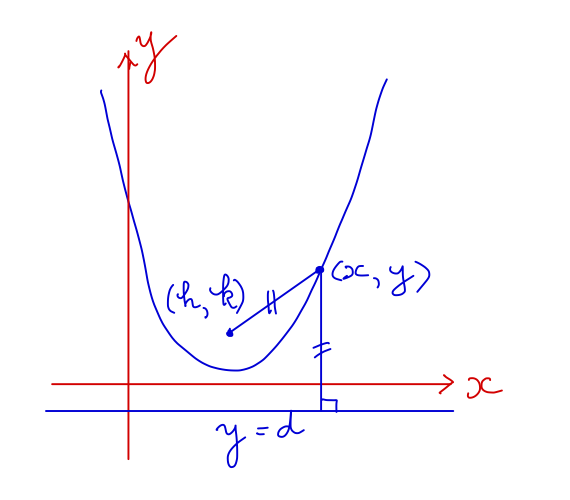
\includegraphics[width=.4\textwidth]{8-1.jpeg} 
\caption{Distance from $ (x,y) $ to the focal point $ (h,k) $ and to the directrix $ y=d $ are equal.}
\label{f:8-1}
\end{center}
\end{figure}


\noindent \textbf{1}  \quad From the definition of focus and directrix, points $ (x,y) $ on the parabola are given by 
\[ (x-h)^2 + (y-k)^2 = (y-d)^2, \]
see Figure~\eqref{f:8-1}.  That is, 
\[  x^2 -2hx + (h^2 +k^2 -d^2) = 2(k-d)y.
\]

This is in the form 
\begin{equation} \label{8fo1} 
2py = x^2 + 2qx + r ,
\end{equation} 
where 
\begin{equation} \label{8a1} 
p= k-d, \quad q=-h, \quad r = h^2 + k^2 -d^2 .
\end{equation} 

\bigskip
\noindent \textbf{2}  \quad
For the parabola $ P $ given by 
\begin{equation} \label{8-P1}  
2py = x^2 + 2qx ,
\end{equation}
we have  $ r=0 $ in \eqref{8fo1}. It follows from~\eqref{8a1} that 
\[
 d^2 = h^2 + k^2 = q^2 + (p+d)^2 = q^2 + p^2 + 2pd + d^2 ,
 \]
 and so 
 \[
 d = -\frac{p^2 + q^2} {2p}, \quad p + d = \frac{p^2 - q^2} {2p}.
 \]
Hence again from~\eqref{8a1}, the focus of $ P $ has coordinates
\begin{equation} \label{8f1} 
 (h,k) =  (-q, p+d) =  \left(-q, \frac{p^2 - q^2} {2p}\right).
\end{equation} 
 

\bigskip
\noindent \textbf{3}  \quad  Let $ P' $ be the parabola
\begin{equation} \label{8-P2} 
2p'x = y^2 + 2q'y.
\end{equation} 
By the previous argument with the roles of $ x $ and $ y $ switched, the focus of $ P' $ has coordinates
\begin{equation} \label{8f2}
(h',k') =  \left( \frac{p'^2 - q'^2} {2p'}, -q' \right).
\end{equation} 

Note that  $ x=0$, $  y=0 $ satisfies \eqref{8-P1} and \eqref{8-P2}, and so the origin $ (0,0 ) $ lies on both $ P $ and $ P' $.
Differentiating both \eqref{8-P1} and \eqref{8-P2} with respect to $ x $, at the origin we find $ \dfrac{dy}{dx} = \dfrac{q}{p} $ for $ P $ and 
$ \dfrac{dy}{dx} = \dfrac{p'}{q'} $ for $ P' $.  

 \begin{figure}[!hbtp]
\begin{center}
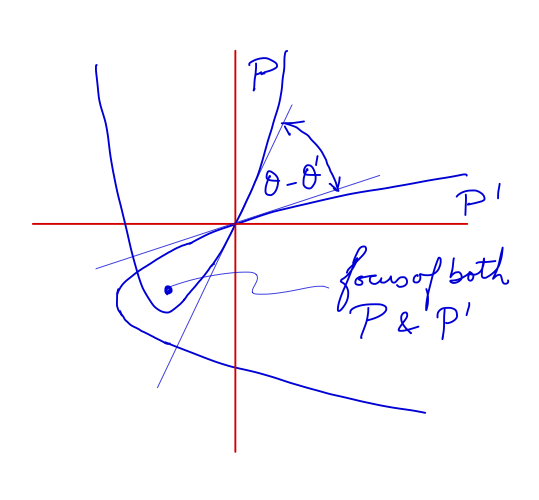
\includegraphics[width=.4\textwidth]{8-2.jpeg} 
\caption{Parabolas with a common focus and orthogonal principal axes.}
\label{f:8-11}
\end{center}
\end{figure}

Let $ \theta $ and $ \theta' $ be the angles that the two tangents at the origin make with the $ x $-axis. Then $ \tan \theta = q/p $ and $ \tan\theta' = p'/q' $.
We want to show that $ \theta - \theta' = \pm \pi/4 $, or equivalently that $ \tan(\theta - \theta' ) = \pm 1 $.
But  
\begin{equation} \label{8-td2}
 \tan(\theta - \theta' )  = \frac{\tan \theta - \tan \theta}{1 + \tan \theta \tan \theta' } = \frac{q/p - p'/q'} {1 + p'q/(pq')} \notag
 	= \frac{q q' - pp' } {pq' + p'q}.
 \end{equation} 
So we want to show 
\begin{align}  \label{}
pq'+ p'q &= \pm (qq' -pp'), \notag \\
\text{equivalently, } (pq'+ p'q)^2 &= (qq' -pp')^2 , \notag \\
\text{equivalently, } 4pp'qq' &= (pp')^2 + (qq')^2 - (pq')^2 - (p'q)^2 .\label{8wr}
\end{align} 

We are given that $ P $ and $ P' $ have the same focus, and so from \eqref{8f1} and \eqref{8f2},
\begin{align*} 
&-q  = \frac{p'^2 - q'^2} {2p'},   \quad  -q' =   \frac{p^2 - q^2} {2p} ,\\
\therefore \quad &-2p'q = p'^2 - q'^2 ,  \quad -2pq' = p^2 -q^2 ,\\
\therefore \quad &4 pp'qq'  =     (pp')^2 + (qq')^2 - (pq')^2 - (p'q)^2 .
\end{align*} 

This establishes \eqref{8wr} and hence that the two tangents at the origin are inclined at $ 45^\circ $.

\bigskip
\noindent \textbf{4}  \quad  The general result is that if two parabolas have orthogonal axes and a common focus, then at each of the two points of intersection their tangents are inclined at $ 45^\circ $ to each other.

\end{proof} 

\bigskip

\paragraph{Tips \& Tricks} The main point is to find an expression for the (tan of the) angle between the two tangent vectors.  See~\eqref{8-td2} and the discussion which precedes it.  The $ \pm $ in the first line of~\eqref{8wr} gives a hint we should square each side of the equality. Then we go back to~\eqref{8f1} and \eqref{8f2} and think about  how we can use the  information there.

%%%%%%%%%%%%%%%%%%%%%%%%%%%%%%%%%%%%%%%%%%%%%%%%%%%%%%%
%%%%%%%%%%%%%%%%%%%%%%%%%%%%%%%%%%%%%%%%%%%%%%%%%%%%%%%%
\newpage
\section*{Question 9}
%\begin{figure}[!hbtp]
\begin{center}
%\includegraphics[width=.5\textwidth]{image7.jpeg} 
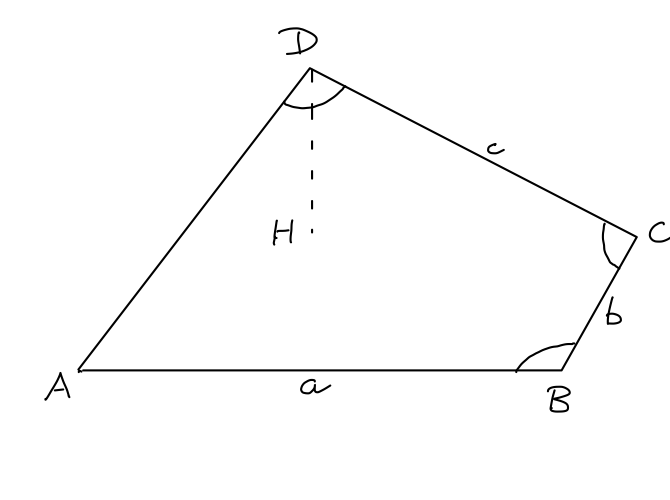
\includegraphics[width=.45\textwidth]{Q9diag.jpeg} 
%\caption{The Allegory of the Cave.  (from Wiki Commons)  }  
\end{center}
%\end{figure}

In the diagram above, which represents a skew quadrilateral ABCD, the angles at B, C, D are right angles.  If H is the foot of the perpendicular from D to the plane ABC, prove that HC is parallel to AB.

If the lengths of AB, BC, CD are respectively a, b, c,  and CD makes an angle $ \alpha $ with the plane ABC, prove that 
\[
c = a \cos \alpha \quad \text{and} \quad AD^2 = a^2 + b^2 - c^2.
\]
Find 
\begin{itemize}[nosep]
\item [(a)] the volume of the tetrahedron ABCD, 
\item [(b)] the perpendicular distance of A from the plane BCD,
\item [(c)] the length of the orthogonal projection of CD on to AB,
\item [(d)] an expression for the angle between the planes  DCA, DCB.
\end{itemize} 

\bigskip



\begin{proof}[Solution] \mbox{}

%\begin{figure}[!hbtp]
\begin{center}
%\includegraphics[width=.5\textwidth]{image7.jpeg} 
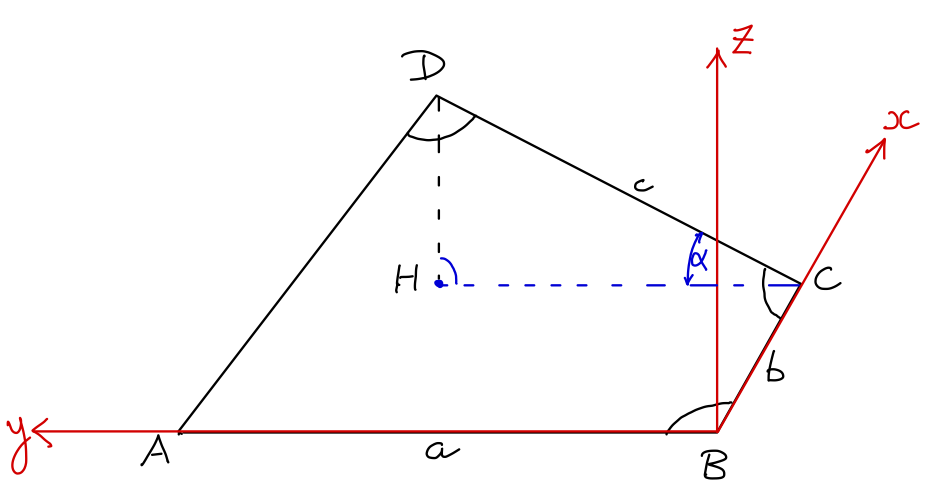
\includegraphics[width=.55\textwidth]{Q9diag2.jpeg} 
%\caption{The Allegory of the Cave.  (from Wiki Commons)  }  
\end{center}
%\end{figure}

Choose cartesian coordinates with   origin at $ B $,   $ x $-axis in   direction $ BC $,    $ y $-axis in   direction $ BA $ and $ z $-axis in the direction given by the right hand thumb rule corresponding to the $ x,y $ axes in that order. 

Then 
\begin{equation} \label{pco}
A= (0,a,0), \quad B = (0,0,0), \quad C = (b,0,0), \quad D= (b, c \cos \alpha , c \sin \alpha ), \quad H = ( b, c \cos \alpha , 0)
\end{equation} 
It follows that 
\begin{equation} \label{vec}
\begin{aligned}
&\overrightarrow{BC} = (b,0,0), \quad \overrightarrow{BA} = (0,a,0), 
\quad \overrightarrow{CD} = (0, c \cos \alpha , c \sin \alpha ), \quad \overrightarrow{AD} = (b, c \cos \alpha -a, c \sin \alpha ),\\
& \overrightarrow{CH}=(0, c\cos \alpha , 0), \quad  \overrightarrow{HD}=(0, c\sin \alpha , 0),
\end{aligned}
\end{equation}

\bigskip 
(i)  $ HC $ is parallel to $ AB $,  since both are parallel to the $ y $-axis from~\eqref{vec}.

\bigskip 
(ii)   Since the angle at $ D $ is a right angle,  $ \overrightarrow{AD} \perp \overrightarrow{CD} $.  Using~\eqref{vec},
\begin{align*}  
0 =  \overrightarrow{AD} \cdot  \overrightarrow{CD} &=  c \cos \alpha (c \cos \alpha - a ) + c^2 \sin^2 \alpha  \\
		&= c^2 -ac\cos \alpha = c (c - a \cos \alpha ) .
\end{align*}   
Since $ c \neq 0 $ it follows that  $ c = a \cos \alpha $.

\bigskip 
(iii)   From~\eqref{vec}
\begin{align*}
{AD^2} &= b^2 +(c \cos \alpha -a)^2 + c^2 \sin^2 \alpha \\
	&= b^2 +c^2 -2ac \cos \alpha + a^2 \\
	&{= a^2 + b^2 -c^2}  \qquad \text{(using (ii))}
\end{align*} 

\bigskip 
(a) The volume of a tetrahedron is $ \frac{1}{3} $  times the area of any side times the perpendicular distance from the opposite vertex to that side. (This is often expresssed as ``$ \frac{1}{3}$  times area of base times height'').  

Hence
\begin{align*}
{  \text{volume of tetrahedron}} & =  \frac{1}{3} \times \text{area}(ABC) \times \text{length} (HD) \\
		&= \frac{1}{3} \cdot \frac{1}{2}ab \cdot c \sin \alpha {  = \frac{abc}{6}  \sin \alpha} .
\end{align*}  

\bigskip 
(b) Since the volume is also $ \frac{1}{3} $ times (the area of $ BCD$)  times (the perpendicular distance of $ A $ from the plane  $ BCD $), it follows from (a) that 
\[
\frac{abc}{6}  \sin \alpha = \frac{1}{3} \times \frac{1}{2} (bc) \times \text{(perp  dist from $ A $ to $ BCD $)}.
\]
Hence the {  perpendicular  distance from $ A $ to $ BCD $ is $ a \sin \alpha $}.

\bigskip 
(c) The orthogonal projection of any point $ P $ onto $ AB $ is given by the $ y $-coordinate of $ P $.  So from~\eqref{pco} the orthogonal projections of $ C $ and $ D $ are $ (0,0,0) $  and $ (0, c\cos \alpha , 0 ) $ respectively.

Hence the {  length of the orthogonal projection of $ CD $ onto $ AB $ is $ c \cos \alpha $}.

\bigskip 
(d) The angle between two planes is the (acute) angle between their normals.  

From~\eqref{vec}, the upward pointing (by the right hand thumb rule) normal to $ DC A    $ is given by 
\begin{align*} 
\overrightarrow{DA} \times \overrightarrow{DC} &= 
	\begin{vmatrix} i & j & k \\ -b & a- c \cos \alpha & -c \sin \alpha  \\ 0 & - c \cos \alpha & - c \sin \alpha \end{vmatrix}\\
	&= i \begin{vmatrix}   a- c \cos \alpha & -c \sin \alpha  \\  - c \cos \alpha & - c \sin \alpha \end{vmatrix}
	  - j \begin{vmatrix}   -b & -c \sin \alpha  \\  0 & - c \sin \alpha \end{vmatrix}
	  + k \begin{vmatrix}   -b & a -c \cos \alpha  \\  0 & - c \cos \alpha \end{vmatrix} \\
	  &= (-ac \sin \alpha , -bc \sin \alpha , bc \cos \alpha ).
\end{align*} 
The squared length of this vector is 
\begin{align*} 
&a^2c^2\sin^2 \alpha + b^2 c^2 \sin^2 \alpha + b^2 c^2 \cos^2 \alpha  = a^2c^2\sin^2 \alpha + b^2 c^2 \\
	&\quad = c^2(a^2 \sin^2 \alpha + b^2 ) = c^2(a^2 - a^2 \cos ^2 \alpha + b^2) = c^2 (a^2 +b^2 - c^2 ),  
\end{align*}
where we used (ii) for the last equality.  Hence the upward pointing unit length vector perpendicular  to $ DC A $    is 
\begin{equation} \label{un1} 
\frac{1}{  \sqrt{a^2 +b^2 -c^2} } (-a  \sin \alpha , -b  \sin \alpha , b  \cos \alpha ).
\end{equation} 

Similarly, the upward pointing normal to $ DC B    $ is given by 
\begin{align*} 
\overrightarrow{CD} \times \overrightarrow{CB} &= 
	\begin{vmatrix} i & j & k \\ 0 &  c \cos \alpha &c \sin \alpha  \\ -b & 0 &0 \end{vmatrix}
	  = (0 , -bc \sin \alpha , bc \cos \alpha ).
\end{align*} 
This has length $ bc $ and so the upward pointing unit length vector perpendicular  to $ DC B $    is 
\begin{equation} \label{un2}
(0 , -  \sin \alpha ,   \cos \alpha ).
\end{equation} 

The scalar product of the two unit length vectors in~\eqref{un1} and~\eqref{un2} is
\[
\frac{b}{ \sqrt{a^2 +b^2 -c^2} },
\]
and so the angle between them, and hence between the planes $ DCA $  and $ DCB $, is 
\[
\cos^{-1} \frac{b}{ \sqrt{a^2 +b^2 -c^2} }.
\]

\end{proof}

\bigskip
\paragraph{Tips \& Tricks} Use Cartesian coordinates.  Choose the origin and    coordinate axes in a manner which simplifies the relevant expessions as much as possible.  Another possibility would be to choose the origin at $ C $ instead of at $ B $.

%%%%%%%%%%%%%%%%%%%%%%%%%%%%%%%%%%%%%%%%%%%%%%%%%%%%%%%
%%%%%%%%%%%%%%%%%%%%%%%%%%%%%%%%%%%%%%%%%%%%%%%%%%%%%%%%
\newpage
\section*{Question 10}

Prove that if the lines $ y=mx $, and $ y = m'x $ harmonically separate $ y=nx$, $ y=n'x $, then
\[
mm' - \frac{1}{2} (m+m')(n+n') +nn' = 0 .
\]
 
 $ y=mx $, $ y=-mx $ are two given fixed lines, and $ H $, $ (h,k)$, and $ H' $, $ (h', k' ) $ are two fixed points.
 
 A point $ P $ moves so that the lines through $ P $ parallel to the fixed lines harmonically separate $ PH $, $ PH' $.  Prove that the locus of $ P $ is a hyperbola, and find the coordinates of its centre, the equations of its principal axes, and its eccentricity.
\bigskip 
\bigskip
\bigskip

\noindent ****************************************
\paragraph{An Aside} 
The notion of ``harmonic separation'' is not standard terminology, and  the corresponding ideas   are not now part of the high school curriculum, so here for context is the relevant background. 

However, the solution of the question requires none  of the following material other than an appropriate choice of line $ L $ in order to compute the cross ratio of the lines $ y=mx ,\  y = m'x $ and $ y=nx,\  y=n'x $.  See Figure~\ref{Q10-2} and the proof of~\eqref{10fde}.

\begin{figure}[!hbtp]
\begin{center}
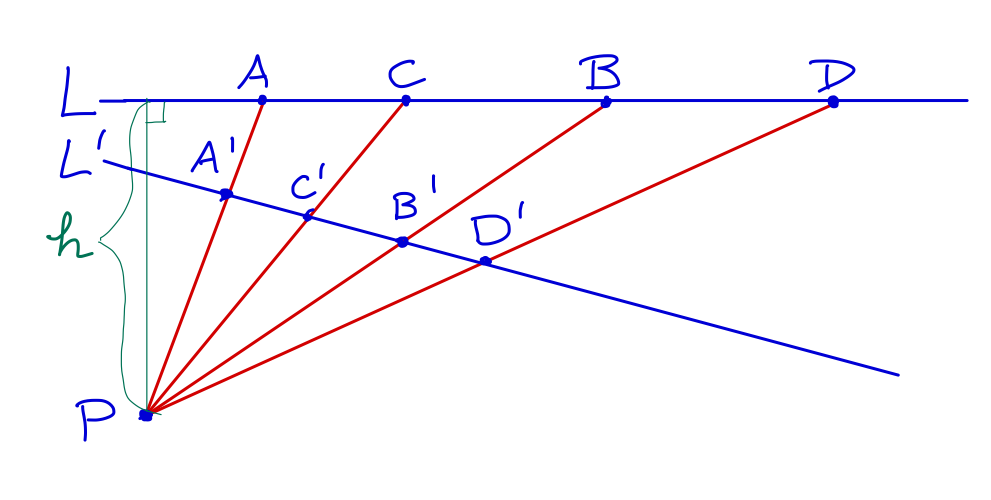
\includegraphics[width=.55\textwidth]{Q10-1.jpeg} 
\caption{$ \frac{AC}{BC} \left/ \frac{AD} {BD}\right. = \frac{A'C'}{B'C'} \left/ \frac{A'D'} {B'D'}\right.  
	= \frac{  \sin \angle APC} { \sin \angle BPC}  \left/ \frac{  \sin \angle APD} { \sin \angle BPD} \right.$ }
\label{Q10-1}
\end{center}
\end{figure}


\noindent \emph{Cross Ratio} \quad Suppose the points $ A, B, C, D $ lie on a straight line $ L $, as in Figure~\ref{Q10-1}.   The \emph{cross ratio}  $ (AB:CD) $ of  the points $  A, B, C, D $ taken in that  order is defined by
\begin{equation} \label{10rel}  
(AB:CD) = \frac{AC}{BC} \left/ \frac{AD} {BD}\right. .
\end{equation} 
 
Here $ AC $, $ BC $, etc. are signed distances.  For example, if the line $ L $ in Figure~\ref{Q10-1} is oriented from left to right then $ AC $ is positive and $ BC $ is negative.

\medskip
\noindent  \emph{Proposition}: \quad  \emph{Suppose  $ P $ is a point not on $ L $, $ L' $ is a second straight line not containing $ P $,   and $ L' $ crosses $ PA, PB, PC, P D$ at $ A', B', C' D' $ respectively.   Then  the corresponding cross ratios for $ L $ and $ L' $ are equal:
\[  
(AB:CD) = (A'B':C'D'), \quad \text{i.e. } \frac{AC}{BC} \left/ \frac{AD} {BD}\right.  =   \frac{A'C'}{B'C'} \left/ \frac{A'D'} {B'D'}\right. .
\]}
Moreover, both equal
\[
\frac{  \sin \angle APC} { \sin \angle BPC}  \left/ \frac{  \sin \angle APD} { \sin \angle BPD} \right. .
\]

\begin{proof} 
Let $ h $ be the perpendicular distance from $ P $ to $ L $, see Figure~\ref{Q10-1}.   Then
\begin{align*} 
\text{area } \triangle PAC &= \frac{1}{2} h \cdot AC = \frac{1}{2} PC \cdot PA\ \sin \angle APC \\
\text{area } \triangle PBC &= \frac{1}{2} h \cdot BC = \frac{1}{2} PC \cdot PB\ \sin \angle BPC \\
\text{area } \triangle PAD &= \frac{1}{2} h \cdot AD = \frac{1}{2} PD \cdot PA\ \sin \angle APD \\
\text{area } \triangle PBD &= \frac{1}{2} h \cdot BD = \frac{1}{2} PD \cdot PB\ \sin \angle BPD  
\end{align*} 
(Here $ \sin \angle APC $ is positive, $ \sin \angle BPC $ is negative, etc.) 
Hence
\begin{align} 
(AB:CD) &= \frac{AC}{BC} \left/ \frac{AD} {BD}\right. \notag\\
	&= \frac{PA \ \sin \angle APC} {PB\ \sin \angle BPC}  \left/ \frac{PA \ \sin \angle APD} {PB\ \sin \angle BPD} \right. \notag\\
	&= \frac{  \sin \angle APC} { \sin \angle BPC}  \left/ \frac{  \sin \angle APD} { \sin \angle BPD} \right. . \notag %\label{10acr}.
\end{align} 
Therefore the cross ratio of the distances equals the ``cross ratio'' of the corresponding angles subtended at $ P $.  But these angles are the same for $ L $ and $ L' $. Hence \mbox{$ (AB:CD) = (A'B':C'D')$}. 
\end{proof} 

\medskip
\noindent  \emph{Definition}: \quad  If $ A, B, C, D $ are on a straight line not containing $ P $, then the points $ \{ A, B \} $ \emph{harmonically separate}  the points $ \{C,D \} $, and the lines $ \{PA, PB\} $ \emph{harmonically separate} the lines $ \{ PC, PD \} $,  if $ (AB:CD) = -1 $.

\medskip
\noindent \emph{Remarks}
\begin{itemize}[nosep]  
\item By the previous Proposition, one can use any line crossing all 4 lines $ \{PA, PB,  PC, PD \} $ and the corresponding intersection points, in order to compute the relevant cross ratio.
\item The significance of $ (AB:CD) = -1 $ is that the points $ C $ and $ D $ divide the line segment $ AB $ internally and externally in the same ratio.  The reason for $ -1 $ and not $ +1 $ is that in the $ +1 $  case it follows that $ C= D $. 
\end{itemize} 

\bigskip
\bigskip

\noindent ****************************************
\begin{proof}[Solution to Question] \mbox{}

\begin{figure}[!hbtp]
\begin{center}
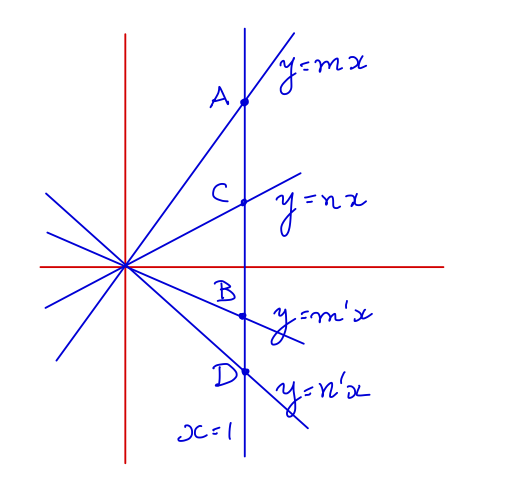
\includegraphics[width=.4\textwidth]{Q10-2.jpeg} 
\caption{$ y=mx $ and $ y = m'x $ harmonically separate $ y=nx$ and $ y=n'x $.}
\label{Q10-2}
\end{center}
\end{figure}

See Figure~\ref{Q10-2}.
Consider the line $ x=1 $.  The lines $ y=mx $,   $ y = m'x $, $ y=nx$  and $ y=n'x $, cross this line at the $ y $-values $ m, m', n, n' $ respectively.
Hence from~\eqref{10rel} with $ A = (1,m) $, $ B = (1,m') $,  $ C = (1,n) $ and $ D = (1,n') $,   and using the definition of ``harmonically separate'',
\begin{align} 
(AB:CD) = \frac{n-m}{n-m'} \left/ \frac{n'-m}{n'-m'}\right. &= -1\notag\\
\therefore \quad (n-m)(n'-m') &= -(n-m')(n'-m)  \notag\\
\therefore \quad  2mm' +2nn' -(mn + mn' + m'n+m'n') &=0\notag\\
\therefore \quad mm' - \frac{1}{2} (m+m')(n+n') +nn' &= 0 \label{10fde}.
\end{align}

\begin{figure}[!hbtp]
\begin{center}
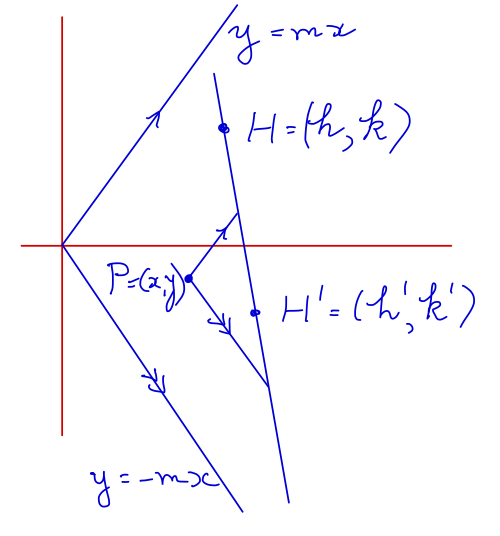
\includegraphics[width=.35\textwidth]{Q10-3.jpeg} 
\caption{The lines through $ P $ with slope $ \pm m $ harmonically separate  $ PH $ and $ P H' $.}
\label{Q10-3}
\end{center}
\end{figure}



See Figure~\ref{Q10-3}.
Let $ P $ have coordinates $ (x,y) $.  Denote the slopes of the lines $ PH $ from $ P $ to $ H $, and  $ PH' $ from $ P $ to $ H' $, by
\[
n = \frac{k-y} {h-x} , \quad n' = \frac{k'-y} {h'-x} ,
\]
respectively. The slopes of the lines parallel to the fixed planes are $ m $ and $ -m $ respectively.

We can apply \eqref{10fde} with $ m,m',n,n' $ there, replaced here by $ m,-m,n,n' $ respectively.  This is justified since translation, in this case moving $ P $ to the origin, does not change the slopes of the four lines through $ P $.  
Note also from~\eqref{10rel} that a pair of lines $ L_1, L_2 $ harmonically separate another pair $ L_3, L_4$ if and only if $ L_3, L_4 $ harmonically separate  $ L_1, L_2$.

This gives  
\begin{align} 
-m^2  +  \frac{k-y} {h-x} \times \frac{k'-y} {h'-x} &= 0 \notag\\
\therefore \quad m^2(x-h)(x-h') &= (y-k)(y-k')  \notag \\
\therefore \quad m^2\left( x^2 - x(h+h') + hh' \right) &=   y^2 - y(k+k') + kk'    \notag \\
\therefore \quad  m^2\left( \left( x - \frac{h+h'} {2} \right)^2  - \left( \frac{h+h'} {2} \right)^2 + hh' \right) 
			      &=    \left( y - \frac{k+k'} {2} \right)^2  - \left( \frac{k+k'} {2} \right)^2 + kk'   \notag \\
\therefore \quad m^2  \left( x - \frac{h+h'} {2} \right)^2 -    \left( y - \frac{k+k'} {2} \right)^2 &=
						\frac{m^2}{4} (h - h')^2 - \frac{1}{4} (k-  k')^2 \label{10nsf}.				
\end{align} 

This is an hyperbola with centre $ \big( (h + h')/2, (k+k')/2 \big) $, and principal axes $ x = \frac{1}{2} (h+h') $ and $ y =  \frac{1}{2} (k+k')   $.

\medskip
The eccentricity of the hyperbola in  the \emph{standard form} $ x^2/a^2 - y^2/b^2 = 1 $ is $ \sqrt{1 + b^2/a^2 } $.
In order to put~\eqref{10nsf} into standard form, let 
\[
\gamma = \frac{m^2}{4} (h - h')^2 - \frac{1}{4} (k-  k')^2  .
\]

We   assume $ \gamma \neq 0 $, since $ \gamma = 0$ implies  $ \dfrac{k-k'}{h-h'} = \pm m $, which   implies $ HH' $ is parallel to one of the two fixed lines, and so the locus of $ P $ is not properly defined.

If $ \gamma > 0 $, then on dividing both sides of~\eqref{10nsf} by $ \gamma $ and translating $\big((h+h')/2, (k+k')\big) $ to the origin, the locus of $ P $ is in standard form with $ a= \sqrt{\gamma}\, m^{-1} $ and $ b  = \sqrt{ \gamma } $. In this case the eccentricity is $ \sqrt{1 + b^2/a^2} = \sqrt{1+m^2 } $. Note that translating to the origin does not change the geometric properties such as eccentricity.

If $ \gamma < 0 $ then, on dividing  by $ - \gamma $ and again translating $\big((h+h')/2, (k+k')\big) $ to the origin, the locus of $ P $ is 
$ y^2/(- \gamma ) - m^2x^2/(- \gamma ) = 1 $.  Switching $ x $ and $ y $  amounts to reflection in the line $ x=y $ and so does not affect the eccentricity.  So the eccentricity is $ \sqrt{1 + \dfrac{(- \gamma ) m^{-2}}{- \gamma } } = \sqrt{1+ m^{-2} }$ .




%in standard form with $ a= \sqrt{ \gamma }  $ and $ b  = \sqrt{\gamma}\, m^{-1}  $. In this case the eccentricity is $ \sqrt{1+m^{-2 }} $.
\end{proof}


\bigskip
\paragraph{Tips \& Tricks} 
\begin{itemize} [nosep]
\item In order to derive~\eqref{10fde} you need to know the meaning of ``harmonically separates''.  But then the derivation is straightforward.
\item The next point is that you should treat $ P $ as the origin in order to derive~\eqref{10nsf}.  This is legitimate since the cross ratio  is invariant under translation. \emph{Why?}
\item Finally, you need to separately consider the cases $ \gamma > 0 $ and  $ \gamma < 0 $ in order to derive the eccentricity.
\end{itemize} 
















\end{document}



